%\documentclass{nitocs}
\documentclass[summary]{nitocs}
% \documentclass[summary,draft]{nitocs} % 画像がコンパイルされない


\usepackage[dvipdfmx]{graphicx}
\usepackage{latexsym}
\usepackage{bm}
\usepackage{amsmath}
\numberwithin{equation}{section}
\graphicspath{{./IMG/}} % 画像指定用のパス

\renewcommand{\theequation}{\arabic{equation}}
\renewcommand{\thefigure}{\arabic{section}.\arabic{figure}}
\renewcommand{\thetable}{\arabic{section}.\arabic{subsection}.\arabic{table}}
\makeatletter
\@addtoreset{equation}{section}
\@addtoreset{figure}{section}
\@addtoreset{table}{section}
\setlength{\mathindent}{0pt}
% 
\def\Underline{\setbox0\hbox\bgroup\let\\\endUnderline}
\def\endUnderline{\vphantom{y}\egroup\smash{\underline{\box0}}\\}
\def\|{\verb|}

\setcounter{page}{1}
\begin{document}

    \title{囲碁における盤面識別システムの検討}
    \author{橋本 燎}{Ryo Hashimoto} % 氏名
    \advisor{井上 優良}{Yusuke Inoue}   % 指導教員氏名

    %! 実行時の日付が自動挿入されるはず
    \date{令和3年\number\month 月\number\day 日} 

    \maketitle
    \section{緒言} \label{intro}
        囲碁は,2人のプレイヤーが碁石を碁盤へ配置するボードゲームである.碁石は各プレイヤーが使用する白黒の石であり,碁盤は通常$19\times19$の格子状の盤面のことを指す.
        %! ルール説明とかで文章を増やそう
        このゲームは両プレイヤーが碁石を交互に碁盤上に設置し,碁石で囲まれた陣地を多く確保したプレイヤーが勝利する.
        相手の陣地として成立している領域でなければどこにでも碁石を置くことができる,相手プレイヤーの碁石を陣地内に収めることでその碁石を奪い使用することで相手陣地の縮小を行うことができる等,
        ルール上の制約が極めて少ないといった特徴を持つため,他のボードゲームと比較すると可能な総局面数は膨大になる.
        % 2016年には$19\times19$の盤面における総局面数の正確な値が計算され,約$2.081681994 \times 10^{170}$通りということが明らかにされた\cite{numbers}.
        % これはオセロや将棋の総局面数を超え,観測可能な宇宙に存在する原子の総数(約$4\times10^{79}$個)よりも遥かに大きな値である.
        
        近年では,2015年にGoogle DeepMind社が開発した,ディープラーニングを実装した囲碁プログラム{\it AlphaGo}\cite{AlphaGo}が初めてプロ棋士に対しハンデ無しの対局で勝利した.
        コンピュータが人間に打ち勝つのは難しいとされていた分野で勝利を果たしたことは,人工知能の有用性を広く知らしめるものとなった.
        以降にも様々な人工知能が登場しプロ棋士との対局が行われてきたが,これらの対局の様子を見ると,プロ棋士の置いた石の配置をコンピュータに入力する役割を持った人間が存在していた.
        そこで,人の手による記録作業を行わずに対局の状況を記録できるシステムの構築を目指す.

        本研究では,対局中の囲碁の画像から碁石の配置を識別するシステムの検討を行う.
        % 段落変更対策
        具体的には,盤面を含む画像から射影変換を用いて盤面を切り抜き,ノイズ処理を適用して盤面上の線を曖昧なものにした後に,輝度値をもとに碁石の配置を識別するシステムの構築を行う.
        その後,複数の画像に対してシステムを試し,結果を考察する.

    \section{理論} \label{theory}
        \subsection{変換}
            \subsubsection{同次座標}
                座標$(x,y)$に対し,その要素を1つ増やした座標$(\xi_1,\xi_2,\xi_3)$を,以下の関係式を満たすように定義する.\\
                \begin{equation} % 同次座標の数式
                    \begin{split} % 複数行に1つの式番号を与える
                        x = \frac{\xi_1}{\xi_3} \\ 
                        y = \frac{\xi_2}{\xi_3}
                    \end{split}
                    \label{Homogeneous}
                \end{equation}

                ただし,$\xi_1,\xi_2,\xi_3$のうち少なくとも1つは0ではないとする.このように定義される座標を同次座標と呼ぶ\cite{DIP}.

                同次座標においては$\lambda\neq0$なる任意の$\lambda$に対して,$(\xi_1,\xi_2,\xi_3)$と$(\lambda\xi_1,\lambda\xi_2,\lambda\xi_3)$は通常の座標に直したときともに$(\xi_1/\xi_3,\xi_2/\xi_3)$となるため,同じ点を表している.つまり,同次座標による表現では,定数倍をしても変わらないとみなすことができる.このような表現を同値であるとよび,これを式では以下のように表す.
                \begin{equation} % 同次座標の数式2
                    \left(
                        \begin{array}{ccc}
                            \xi_1\\
                            \xi_2\\
                            \xi_3
                        \end{array}
                    \right) \sim % \sim: 「~」
                    \left(
                        \begin{array}{ccc}
                            \lambda\xi_1\\
                            \lambda\xi_2\\
                            \lambda\xi_3
                        \end{array}
                    \right)
                \end{equation}
                ここで記号$\sim$は同値関係を表し,定数倍の違いを許して等しいことを意味する.

            \subsubsection{射影変換}
                同次座標を利用することにより,一般的な変換を表現することができる.
                これは以下の式で表現されるもので,射影変換と呼ばれている\cite{DIP}.
                \begin{equation} % 射影変換の数式
                    \left(
                        \begin{array}{ccc}
                        x'\\
                        y'\\
                        1
                        \end{array}
                    \right)\sim
                    \left(
                        \begin{array}{ccc}
                        h_{11} & h_{12} & h_{13}\\
                        h_{21} & h_{22} & h_{23}\\
                        h_{31} & h_{32} & h_{33}\\
                        \end{array}
                    \right)
                    \left(
                        \begin{array}{ccc}
                        x\\
                        y\\
                        1
                        \end{array}
                    \right)
                    \label{Homography}
                \end{equation}

                射影変換においては,線分の直線性は保たれるものの,平行性は失われる.別の言い方をすると,任意の四角形を別の任意の四角形に移すような変換であるといえる.
                    %? 「概略図」? なんかパッとしない表現
                射影変換の概略図を図\ref{sample_homography}に示す.
                \begin{figure}[tb] % 射影変換の概略図
                    \begin{center}
                    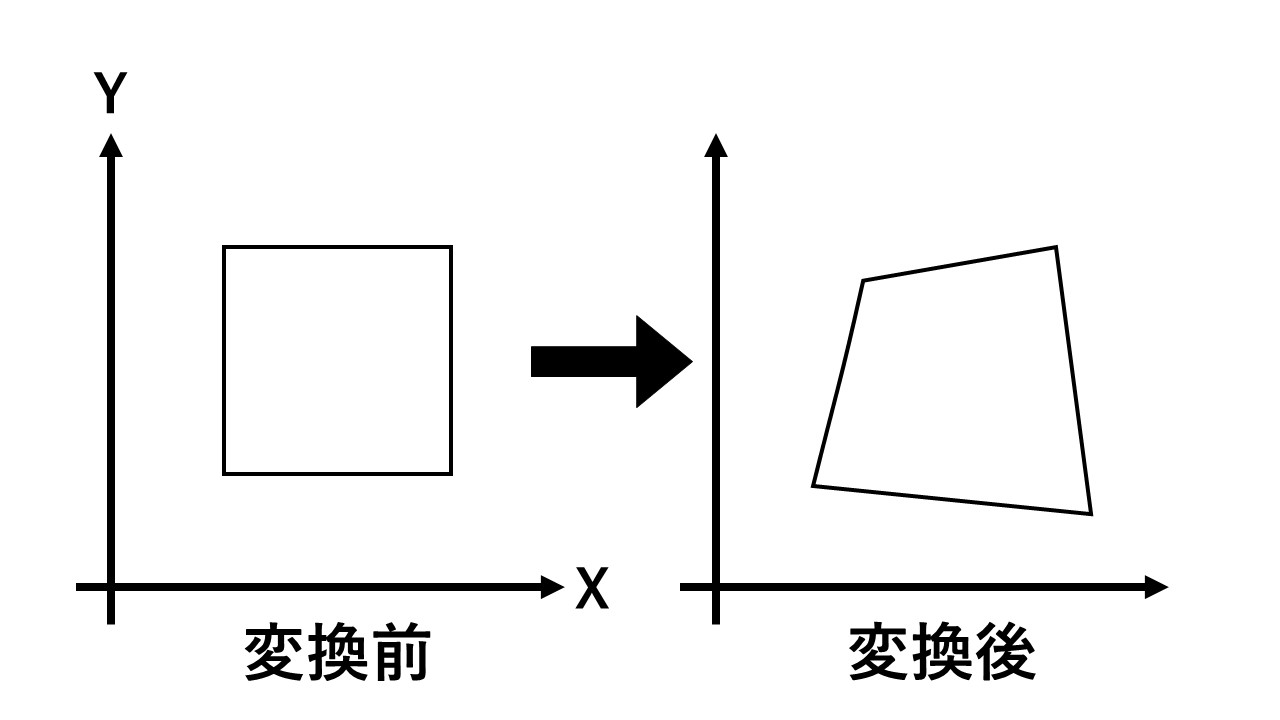
\includegraphics[clip,width=80mm]{Homography.jpg} 
                    \caption{射影変換の概略図}
                    \label{sample_homography}
                    \end{center}
                \end{figure}

%4
    \section{システム内容} \label{system}
        システムは,与えられた画像に対して,以下の前処理を行う.
        \begin{itemize}
            \item 射影変換(盤面部分の切り抜き)
            \item グレースケール化
            \item ノイズ処理
        \end{itemize}
        前処理が完了した画像に対して,システムは$19\times19$個の小さな領域を付与する.
        この領域内に存在する画素値の平均と,設定したしきい値をもとに,システムは各領域の位置に置かれている石の種類の識別を行う.
            %TODO 必要であれば領域付与済みの図を入れる

    \section{実験} \label{experiment}
        じっけん

    \section{結言}\label{conclusion}
        けつげん


    \begin{thebibliography}{10}
        %! 参考文献
        \bibitem{AlphaGo}
        DeepMind「AlphaGo | DeepMind」(最終閲覧日:令和3年1月13日)
        
        https://deepmind.com/research/case-studies/alphago-the-story-so-far

        \bibitem{DIP}
        ディジタル画像処理[改訂第二版],松阪 喜幸(2020)
    \end{thebibliography}

\end{document}
